\section{System for elektroniske kalendre}
\subsection{Oversikt over systemet}

Hver ansatt i Firma X skal ha en personlig kalender. Hver gruppe skal ha en gruppe kalender. En gruppe kan bestå av flere personer og også av subgrupper. En person kan være medlem av flere grupper. Alle kalenderne skal være lagret på en kalendertjener. De ansatte skal ha tilgang til kalenderne sine med en kalenderklient. Kalenderklienten kjører på en lokalmaskin som kommuniserer med kalendertjeneren over lokalnettet. Mange kalenderklienter kan være koblet opp mot kalendertjeneren samtidig. Sammen utgjør kalendertjeneren og kalenderklientene systemet som skal implementeres.
Figur \ref{fig:high-level-architecture}  viser et høynivå systemarkitektur over kalendersystemet.

\begin{figure}[H]
    \centering
    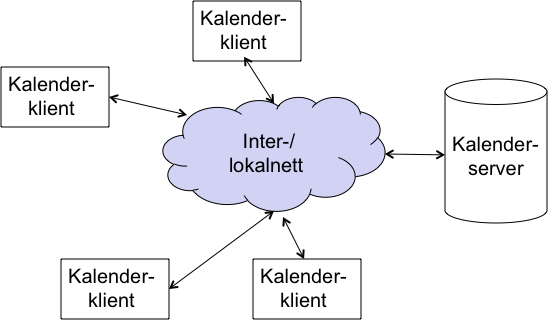
\includegraphics[scale=0.5]{resources/high-level-architecture.png}
    \caption{High level system architecture for calendar system}
    \label{fig:high-level-architecture}
\end{figure}

\subsection{Scenarioer}

Scenarioene er ikke en del av kravspesifikasjonen, men skisserer noen typiske bruksscenarier for kalendersystemet, som vil støttes dersom kravene oppfylles.

\begin{enumerate}

\item
Per har invitert tre forretningsforbindelser til samtaler i egne lokaler førstkommende fredag klokka 12 til 14. Per legger inn dette som en avtale i kalenderen sin, legger inn kollegaen Siv som deltaker (han ser hun er ledig da) og får kalendersystemet til å booke et ledig møterom som er passe stort for fem deltakere.

\item
Siv får en telefon om at hun må delta på et møte hos et eksternt møte hos en oppdragsgiver. Mens hun prater i telefonen, legger hun møtet inn i kalenderen sin. Hun ser at det overlapper med møtet som Per har lagt henne inn i, og siden det eksterne møtet har prioritet, så går hun inn på gruppemøtet og markerer at hun ikke kan delta.

\item
Per ser at det dukker opp et varsel om at Siv har angitt at hun ikke kan delta, så han sletter henne og legger inn Beate istedet. Beate får på sin side dette opp som et møteforslag i sin kalender og bekrefter at hun kan stille.

\item
En av de tre forretningsforbindelsene ringer og sier at alle tre blir forsinket med én time. Per angir dette i møteinnkallingen og siden systemet viser at møterommet som var booket, er opptatt da, så ber han systemet om å finne et nytt. Beate får melding om endringen, og forholder seg til det, men siden hun er på farta så sender hun en tekstmelding om at det går greit. Per markerer da for henne at hun kommer.

\end{enumerate}

\subsection{Krav til kalendersystemet}

I tillegg til at de ansatte skal kunne planlegge dagene sine med å legge inn avtaler i kalenderne, er hensikten med kalendersystemet å forenkle innkalling til møter. I dag bruker de ansatte i Firma X mye tid på å koordinere intern-møter i organisasjonen. Tiden går med på å finne tidspunkt som passer for alle møtedeltakere, samt å reservere møterom. Kalendersystemet skal administrere innkalling til møter og reservasjon av møterom.

\begin{enumerate}

\item
Logge på. Ansatte får tilgang til kalendersystemet ved å logge seg på kalenderklienten med brukernavn og passord.

\item
Legge inn avtale. Ansatte skal kunne legge inn avtaler i kalenderen sin. En avtale legges inn på avtaledato med et start- og sluttidspunkt alternativt start-tidspunkt og varighet, samt en kort beskrivelse av avtalen ("Bil på verksted") og eventuelt sted for avtalen ("Strandveien
>Auto"). Det skal være lov å legge inn flere avtaler for overlappende tidspunkt.

\item
Håndtere møtedeltakere. Den som har lagt til en avtale skal også kunne legge til (eller fjerne) (potensielle) deltakere, ved å angi enkeltpersoner og/eller grupper. Grupper administreres utenfor systemet og kan ses på som en samling personer uten noen spesiell struktur (roller/hierarkier). Inviterte deltakerne skal kunne bekrefte evt. avkrefte at de deltar. Dersom en deltaker avkrefter deltakelse, så kan han/hun også velge om den skal skjules i kalenderen sin.

\item
Endre avtale. Ansatte skal kunne endre på avtaler de har opprettet. Alle feltene kan endres. Alle deltakere blir varslet om endringen (på en eller annen måte), så de kan forholde seg til det og evt. endre på om de deltar eller ikke.

\item
Slette avtale. Ansatte skal kunne slette avtaler de har opprettet, og disse forsvinner da fra kalenderen til alle deltakere.

\item
Reservere møterom. I stedet for å skrive inn sted for en avtale eller et møte, skal brukeren kunne velge møterom blant de som er ledige i det angitte tidsrommet. Ved endring av tidsrommet, skal kalendersystemt automatisk reservere møterommet for det nye tidrommet, men ikke holde på
>det om andre har reservert det da. Det skal være mulig å angi antall deltakere som rommet skal kunne ta, uavhengig av antallet deltakere som er invitert og evt. har bekreftet at de kommer.

\item
Visning. Kalenderklienten skal vise en ukeoversikt der alle avtaler og møter i den ansattes personlige kalender vises. Det skal være et tydelig skille mellom avtaler som en har opprettet selv og avtaler som en er invitert til. For avtaler en er invitert til så skal det være tydelig angitt status for egen deltakelse (om en har bekreftet/avkreftet deltakelsen). Det skal være tydelig angitt om en avtale er endret, så brukeren kan forholde seg til endringen. (Merk at det ikke er definert hva som gjør at systemet tror brukeren har forholdt seg til endringen.)

\item
Status for deltakelse. For møter med inviterte deltakere så skal det være tydelig angitt om 1) en alle har svart eller ikke og 2) om det er noen som har avslått invitasjonen.

\item
Melde avbud for møte. En ansatt kan melde avbud på en møteinnkalling ved å slette avtalen i sin personlige kalender. Når en ansatt melder avbud, sendes melding til alle de andre møtedeltakerne. Møteleder kan da velge om møtet skal avlyses eller om han/hun skal endre tidspunkt på møtet.

\item
Reservere møterom. I stedet for å skrive inn sted for en avtale eller et møte, skal brukeren kunne reservere møterom. Kalendertjeneren skal lage en liste med tilgjengelige møterom (tilgjengelig betyr ikke reserverte) i tidsperioden for avtalen/møtet. Brukeren kan da velge møterom fra denne listen. Om en avtale med reservert møterom slettes, skal reservasjonen slettes på kalendertjeneren. Det samme gjelder for møter som avlyses.

\item
Visning. Kalenderklienten skal vise en ukekalender der alle avtaler og møter i den ansattes personlige kalender vises. Det skal være enkelt å bla mellom ukene.

\item
Spore møteinnkallinger. Kalenderklienten skal indikere i ukekalenderen om a) en møteinnkalling venter på svar fra en eller flere deltakere, b) en eller flere møtedeltakere har avslått møteinnkalling, eller c) om alle innkalte har godtatt møteinnkallingen.

\item
Vis flere kalendre. Det skal være mulig å se kalendre (avtaler og møter) for flere ansatte i samme ukesoversikt.

\item
Alarm. Det skal være mulig for hver ansatt å konfigurere enhver avtale slik at avtalen genererer en alarm en gitt tid før møtet. 

\end{enumerate}
